
% Template for Elsevier CRC journal article
% version 1.1 dated 16 March 2010

% This file (c) 2009-10 Elsevier Ltd.  Modifications may be freely made,
% provided the edited file is saved under a different name

% This file contains modifications for Nuclear Physics B Proceedings Supplement

% Changes since version 1.0
% - elsarticle class option changed from 1p to 3p (to better reflect CRC layout)
%

%-----------------------------------------------------------------------------------

%% This template uses the elsarticle.cls document class and the extension package ecrc.sty
%% For full documentation on usage of elsarticle.cls, consult the documentation "elsdoc.pdf"
%% Further resources available at http://www.elsevier.com/latex

%-----------------------------------------------------------------------------------

%%%%%%%%%%%%%%%%%%%%%%%%%%%%%%%%%%%%%%%%%%%%%%
%%%%%%%%%%%%%%%%%%%%%%%%%%%%%%%%%%%%%%%%%%%%%%
%%                                          %%
%% Important note on usage                  %%
%% -----------------------                  %%
%% This file must be compiled with PDFLaTeX %%
%% Using standard LaTeX will not work!      %%
%%                                          %%
%%%%%%%%%%%%%%%%%%%%%%%%%%%%%%%%%%%%%%%%%%%%%%
%%%%%%%%%%%%%%%%%%%%%%%%%%%%%%%%%%%%%%%%%%%%%%

%% The '3p' and 'times' class options of elsarticle are used for Elsevier CRC
\documentclass[3p,times,twocolumn]{elsarticle}

%% The `ecrc' package must be called to make the CRC functionality available
\usepackage{ecrc}

%% The ecrc package defines commands needed for running heads and logos.
%% For running heads, you can set the journal name, the volume, the starting page and the authors

%% set the volume if you know. Otherwise `00'
\volume{00}

%% set the starting page if not 1
\firstpage{1}

%% Give the name of the journal
\journalname{Nuclear Physics B Proceedings Supplement}

%% Give the author list to appear in the running head
%% Example \runauth{C.V. Radhakrishnan et al.}
\runauth{}

%% The choice of journal logo is determined by the \jid and \jnltitlelogo commands.
%% A user-supplied logo with the name <\jid>logo.pdf will be inserted if present.
%% e.g. if \jid{yspmi} the system will look for a file yspmilogo.pdf
%% Otherwise the content of \jnltitlelogo will be set between horizontal lines as a default logo

%% Give the abbreviation of the Journal.
\jid{nuphbp}

%% Give a short journal name for the dummy logo (if needed)
\jnltitlelogo{Nuclear Physics B Proceedings Supplement}

%% Hereafter the template follows `elsarticle'.
%% For more details see the existing template files elsarticle-template-harv.tex and elsarticle-template-num.tex.

%% Elsevier CRC generally uses a numbered reference style
%% For this, the conventions of elsarticle-template-num.tex should be followed (included below)
%% If using BibTeX, use the style file elsarticle-num.bst

%% End of ecrc-specific commands
%%%%%%%%%%%%%%%%%%%%%%%%%%%%%%%%%%%%%%%%%%%%%%%%%%%%%%%%%%%%%%%%%%%%%%%%%%

%% The amssymb package provides various useful mathematical symbols
\usepackage{amssymb}
%% The amsthm package provides extended theorem environments
\usepackage{amsthm}
\usepackage{amsmath}
\usepackage{subfigure}
\usepackage{float}
\usepackage{enumitem}
%% The lineno packages adds line numbers. Start line numbering with
%% \begin{linenumbers}, end it with \end{linenumbers}. Or switch it on
%% for the whole article with \linenumbers after \end{frontmatter}.
%% \usepackage{lineno}

%% natbib.sty is loaded by default. However, natbib options can be
%% provided with \biboptions{...} command. Following options are
%% valid:

%%   round  -  round parentheses are used (default)
%%   square -  square brackets are used   [option]
%%   curly  -  curly braces are used      {option}
%%   angle  -  angle brackets are used    <option>
%%   semicolon  -  multiple citations separated by semi-colon
%%   colon  - same as semicolon, an earlier confusion
%%   comma  -  separated by comma
%%   numbers-  selects numerical citations
%%   super  -  numerical citations as superscripts
%%   sort   -  sorts multiple citations according to order in ref. list
%%   sort&compress   -  like sort, but also compresses numerical citations
%%   compress - compresses without sorting
%%
%% \biboptions{comma,round}

% \biboptions{}

% if you have landscape tables
\usepackage[figuresright]{rotating}
\setlength\parindent{0pt}
%\setlist[enumerate]{leftmargin=*}
% put your own definitions here:
%   \newcommand{\cZ}{\cal{Z}}
%   \newtheorem{def}{Definition}[section]
%   ...

% add words to TeX's hyphenation exception list
%\hyphenation{author another created financial paper re-commend-ed Post-Script}

% declarations for front matter

\begin{document}

\begin{frontmatter}

%% Title, authors and addresses

%% use the tnoteref command within \title for footnotes;
%% use the tnotetext command for the associated footnote;
%% use the fnref command within \author or \address for footnotes;
%% use the fntext command for the associated footnote;
%% use the corref command within \author for corresponding author footnotes;
%% use the cortext command for the associated footnote;
%% use the ead command for the email address,
%% and the form \ead[url] for the home page:
%%
%% \title{Title\tnoteref{label1}}
%% \tnotetext[label1]{}
%% \author{Name\corref{cor1}\fnref{label2}}
%% \ead{email address}
%% \ead[url]{home page}
%% \fntext[label2]{}
%% \cortext[cor1]{}
%% \address{Address\fnref{label3}}
%% \fntext[label3]{}

\dochead{}
%% Use \dochead if there is an article header, e.g. \dochead{Short communication}

\title{Space Weather Alerts for Air Navigation}

%% use optional labels to link authors explicitly to addresses:
%% \author[label1,label2]{<author name>}
%% \address[label1]{<address>}
%% \address[label2]{<address>}

\author[UIS]{Sergio Pinilla}
\author[UIS,CAB]{Hern\'an Asorey}
\author[UIS]{Luis N\'u\~nez}

\address[UIS]{Escuela de f\'isica, Universidad Industrial de Santander, Bucaramanga, Colombia}
\address[CAB]{DPRLab, Centro At\'omico Bariloche \& Instituto Balseiro, Bariloche, Argentina}

\begin{abstract}
%% Text of abstract
The aim of this work is to determine the total integrated flux of cosmic radiation which a commercial aircraft is exposed to along specific flight trajectories. Selection of these trajectories is based on its utilization and geomagnectical effects along them, for example the South Atlantic Anomaly. In order to study the radiation background during a flight and its modulation by effects such as altitude, latitude, exposure time and solar events, we perform simulations  based on codes \textit{Magnetocosmics} and \textit{CORSIKA}, the former designed to calculate the geomagnetical effects on cosmic rays propagation and the latter allows us to simulate the development of extended air showers. Considering the energy range for primary particles from 5 Gev to 1 Pev, we obtain the total flux of secondary particles by means of point-to-point numerical integration.
\end{abstract}

\begin{keyword}
%% keywords here, in the form: keyword \sep keyword
Cosmic rays \sep aircraft \sep CORSIKA \sep Magnetocosmics
%% MSC codes here, in the form: \MSC code \sep code
%% or \MSC[2008] code \sep code (2000 is the default)
\end{keyword}

\end{frontmatter}

%%
%% Start line numbering here if you want
%%
% \linenumbers

%% main text
\section{Introduction}
\label{sec:introduction}
The Earth is constantly being bombarded by subatomic particles which come from the Sun, the Milky Way and extragalactic sources. These particles, known as \textit{primaries}, reach our planet with energies that vary over a wide range: it begins at $10^5$ eV for particles from solar wind and ends beyond $10^{20}$ eV for intergalactic particles. The lower energy primaries are deflected by  Earth's magnetosphere, but the higher energy ones penetrate the atmosphere colliding with atoms in the air and
generating a cascade of \textit{secondary particles}. As altitude increases, the atmosphere protective layer becomes thinner and less dense, that's why the incidence of cosmic radiation on an airplane flying between $10$ km - $12$ km is much higher than at ground levels. Besides altitude, there are other factors that may affect the dose received, such as latitude, space weather, and time of exposure. This phenomenon has been investigated only in the last two decades and it has become an occupational health issue in some countries (see, for example \cite{bottollier-depois_comparison_2012}). To calculate the number of particles incident on an aircraft flying several routes, simulations will be performed using \textit{CORSIKA} and \textit{Magnetocosmics}. \textit{CORSIKA} (COsmic Ray SImulations for KAscade) \cite{heck_extensive_2010} is a detailed Monte Carlo program to study the evolution and properties of extensive air showers in the atmosphere. \textit{Magnetocosmics} \cite{desorgher_magnetocosmics_2006} is a code based on Geant4 that allows to calculate the trajectories of charged particles through different geomagnetic field models.
\section{Rigidity of a particle}
\label{sec:rigidity_particle}
The motion of a charged particle through a magnetic field is described by the relativistic Lorentz equation of motion:
\begin{equation}
\frac{d\boldsymbol{\vec{p}}}{dt}=\frac{q}{c}\boldsymbol{\vec{v}}\times\boldsymbol{\vec{B}}
\end{equation}
This equation of motion conserves the magnitude of the momentum $p$, and therefore the energy of the particle. After some transformations, it becomes:
\begin{equation}
\frac{d\boldsymbol{\hat{I}_v}}{ds}=\frac{q}{pc}\boldsymbol{\hat{I}_v}\times\boldsymbol{\vec{B}}
\end{equation}
where $\boldsymbol{\hat{I}_v}$ is the unit vector in the direction of velocity and $s$ is the path length along the particle trajectory. The rigidity of the particle is defined by:
\begin{equation}
R=\frac{pc}{q}
\end{equation}
And it is a measure of the resistance of the particle to the bending of its trajectory by the magnetic field.
\subsection*{\textbf{Rigidity cut-off}}
%\label{sec:rigidity_cut_off}
It is the lower rigidity limit above which cosmic rays can cross the Earth magnetosphere and reach a specific position from a specific observational direction. It depends on the geographical coordinates and on particle's direction of arrival.
\section{Earth magnetic field models}
\label{sec:Earth_geomagnetic_models}
\subsection*{\textbf{Internal field ($\boldsymbol{r<5R_E}$)}}
The International Geomagnetic Reference Field (IGRF) \cite{susan_macmillan_international_2010} is an internationally agreed and widely used mathematical model of the Earth magnetic field of internal origin. In this model:
\begin{equation}
\boldsymbol{\vec{B}}=-\boldsymbol{\vec{\nabla}}V\qquad\nabla^2V=0
\end{equation}
Each constituent model of the IGRF is a set of spherical harmonics of degree $n$ and order $m$, representing a solution to Laplace's equation for the magnetic potential arising from sources inside the Earth at a given epoch; the harmonics are associated with the Gauss coefficients $g_n^m$ and $h_n^m$:
\begin{multline}
V(r,\theta,\lambda)=a\sum_{n=1}^{n_{max}}\left(\frac{a}{r}\right)^{n+1}\sum_{m=0}^n\left(g_n^m\cos m\lambda\right.\\
\left.+h_n^m\sin m\lambda\right)P_n^m(\theta)
\end{multline}

\subsection*{\textbf{External field ($\boldsymbol{r>5R_E}$)}}
Beyond five Earth radii, the Earth magnetic field is increasingly affected by the solar wind interaction with the Earth magnetosphere. The distortions can be described by several external source fields caused by magnetospheric current systems.

The Tsyganenko model \cite{woodfield_comparison_2007} is a semi-empirical best-fit representation for the magnetic field, based on a large number of satellite observations (IMP, HEOS, ISEE, POLAR, Geotail, etc). The model includes the contributions from external magnetospheric sources: ring current, magnetotail current system, magnetopause currents and large-scale system of field-aligned currents.

\section{Strategy}
\label{sec:strategy}
\begin{enumerate}[leftmargin=*]
%\item Determination of energy limits: the maximum energy considered is $1PeV$ since the probability of finding a primary particle with this energy is really low during the time of a flight; the lower limit of the energy depends on the geographical location and it's determined using \textit{Magnetocosmics.}
%\item Simulation of showers at one specfic altitude, longitude, latitude  and a very low rigidity cut-off. Simulations are made using \textit{CORSIKA}. 
\item Simulation of showers at a specific site (longitude, latitude, altitude) using \textit{CORSIKA}. Features of injected primaries at the top of the atmosphere:
\begin{itemize}[leftmargin=*]
\item Nuclei considered: $1\leq Z_p\leq 26$, $1\leq A_p\leq 56$
\item  Very low cut-off rigidity: $R_c=4GV$
\item Energy and direction of arrival: $(R_c\times Z_p)\leq (E_p/GeV)\leq 10^6$, $0^\circ\leq\theta_p\leq 90^\circ$, $0^\circ\leq\phi_p\leq 360^\circ$
%\item Direction of arrival: $0^\circ\leq\theta\leq 90^\circ$, $0^\circ\leq\phi\leq 360^\circ$
\item Simulation time: $t=7200 s$ (primary particles flux is constant and isotropic)
\end{itemize}
\item Selection and discretization of routes.
\item Computation of cut-off rigidities for each point in the trajectory using \textit{Magnetocosmics}.
\item Filter of the first simulated showers according to the cut-off rigidities computed for each point of the trajectory: showers generated by primary particles with rigidities below the cut-off rigidities are discarded.
\item Computation of the total amount of particles that hit the aircraft. This is done asuming a constant flux of secondaries on each interval of the trajectory and adding them together.
\item To consider diferent magnetospheric conditions, it is possible to vary the DST index (Disturbance Storm Index).
\end{enumerate}

\section{First results}
\label{sec:first_results}
%In order to study the effect of altitude on the flux of secondary particles we simulated the 
The trajectory chosen was Bogot\'a - Buenos Aires, this route was divided into $12$ intervals of equal flight time and the flux of secondaries along each of them was assumed to be constant and equal to the flux in the midpoint (blue dots). Takeoff and landing was not included in this preliminar analysis and the aircraft was supposed to fly at a constant altitude of $11$ km along the whole trajectory. The data used corresponds to flight ARG1361, made on 24-11-2014. To study the effect of geomagnetic field on the flux of particles and as a way to validate simulations, we calculated the spectrum of secondary particles when geomagnetic field was present and when it was not (figures \ref{fig:geo_effect1} and \ref{fig:geo_effect2}). We noted, as expected, that there is a significant reduction of the flux for low energies when the field is taken into account. In figure \ref{fig:distribution_bta_bsas} it is shown the distribution of particles along the whole trajectory and in figure \ref{fig:integrated_bta_bsas} it is possible to compare the flux of particles when being on the ground with the flux when being on an airplane.

%\begin{figure}[H!]
%\centering
%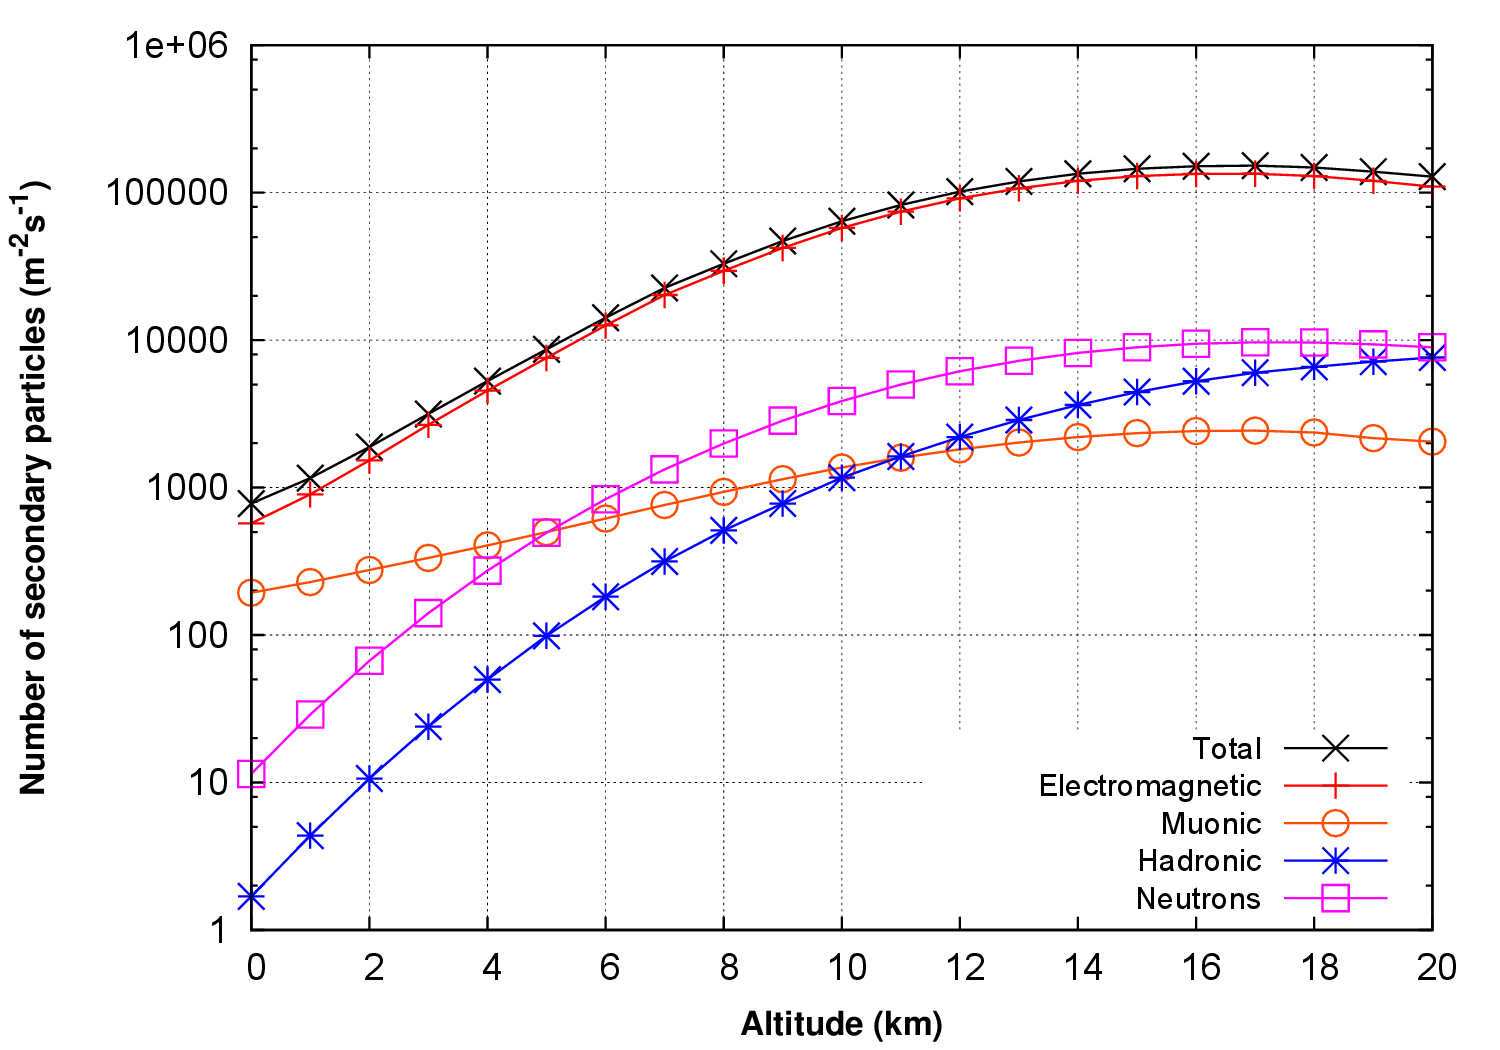
\includegraphics[scale=.15]{figures/componentes2.png}
%\caption{\textit{Flux of particles as function of altitude in Bucaramanga ($7^\circ 07'N\;73^\circ 07'W,\;h_0=1000\;m.a.s.l.$)}}
%\label{fig:altura_hess_kolhorster}
%\end{figure}

%\begin{figure}[H]
%\centering
%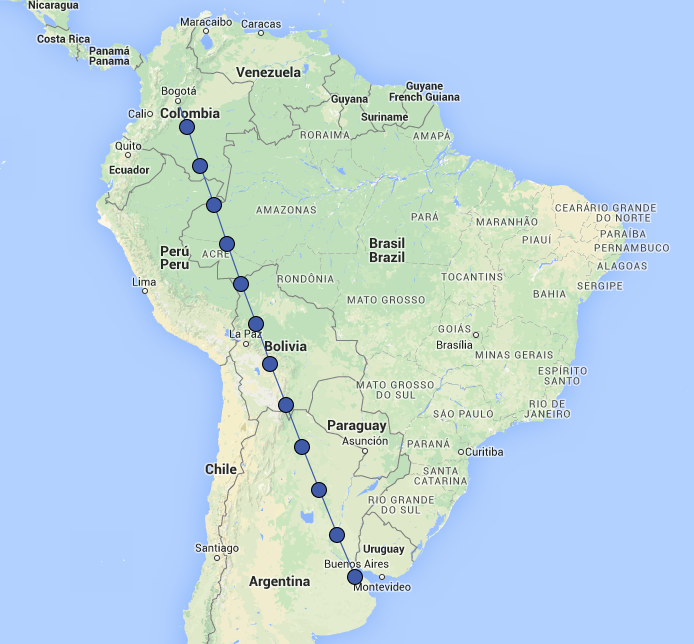
\includegraphics[scale=.17]{figures/bta_bsas.png}
%\caption{\textit{Route Bogot\'a - Buenos Aires.}}
%\label{fig:ruta_bog_bsas}
%\end{figure}
\begin{figure}[H]
\centering
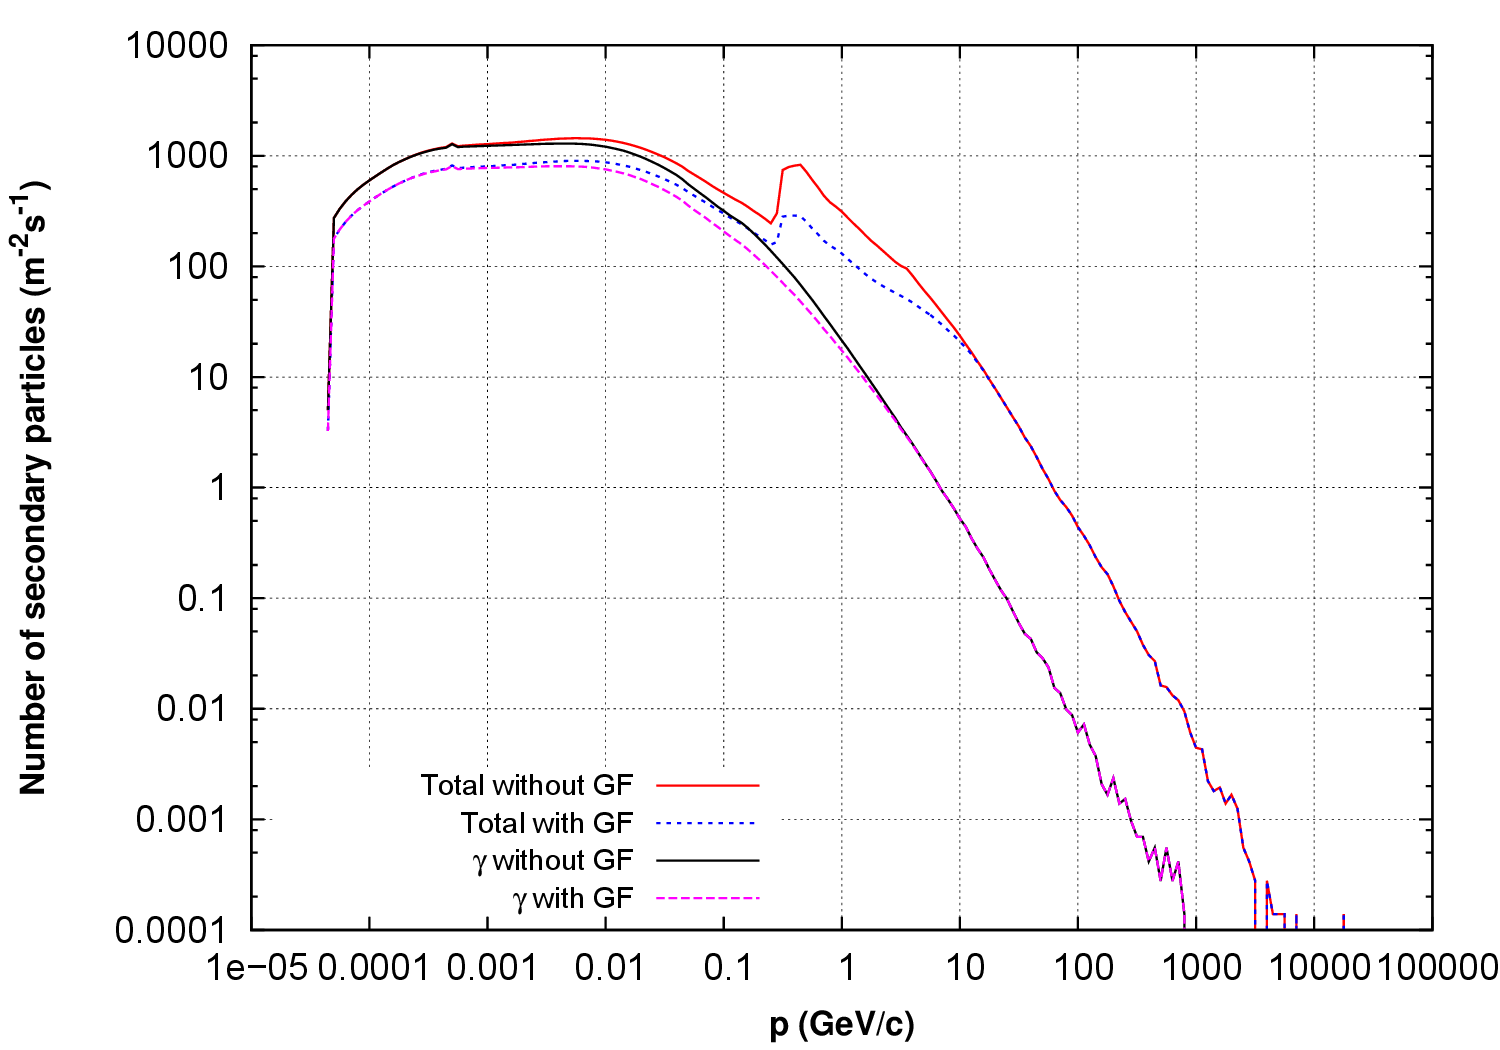
\includegraphics[scale=.14]{figures/g2_efectogeo.png}
\caption{\textit{Distribution of particles considering the Geomagnetic Field  (dashed lines) and not considering it (continuous lines). Location: $14.74^\circ S\;67.27^\circ W$.  }}
\label{fig:geo_effect1}
\end{figure}
\begin{figure}[H]
\centering
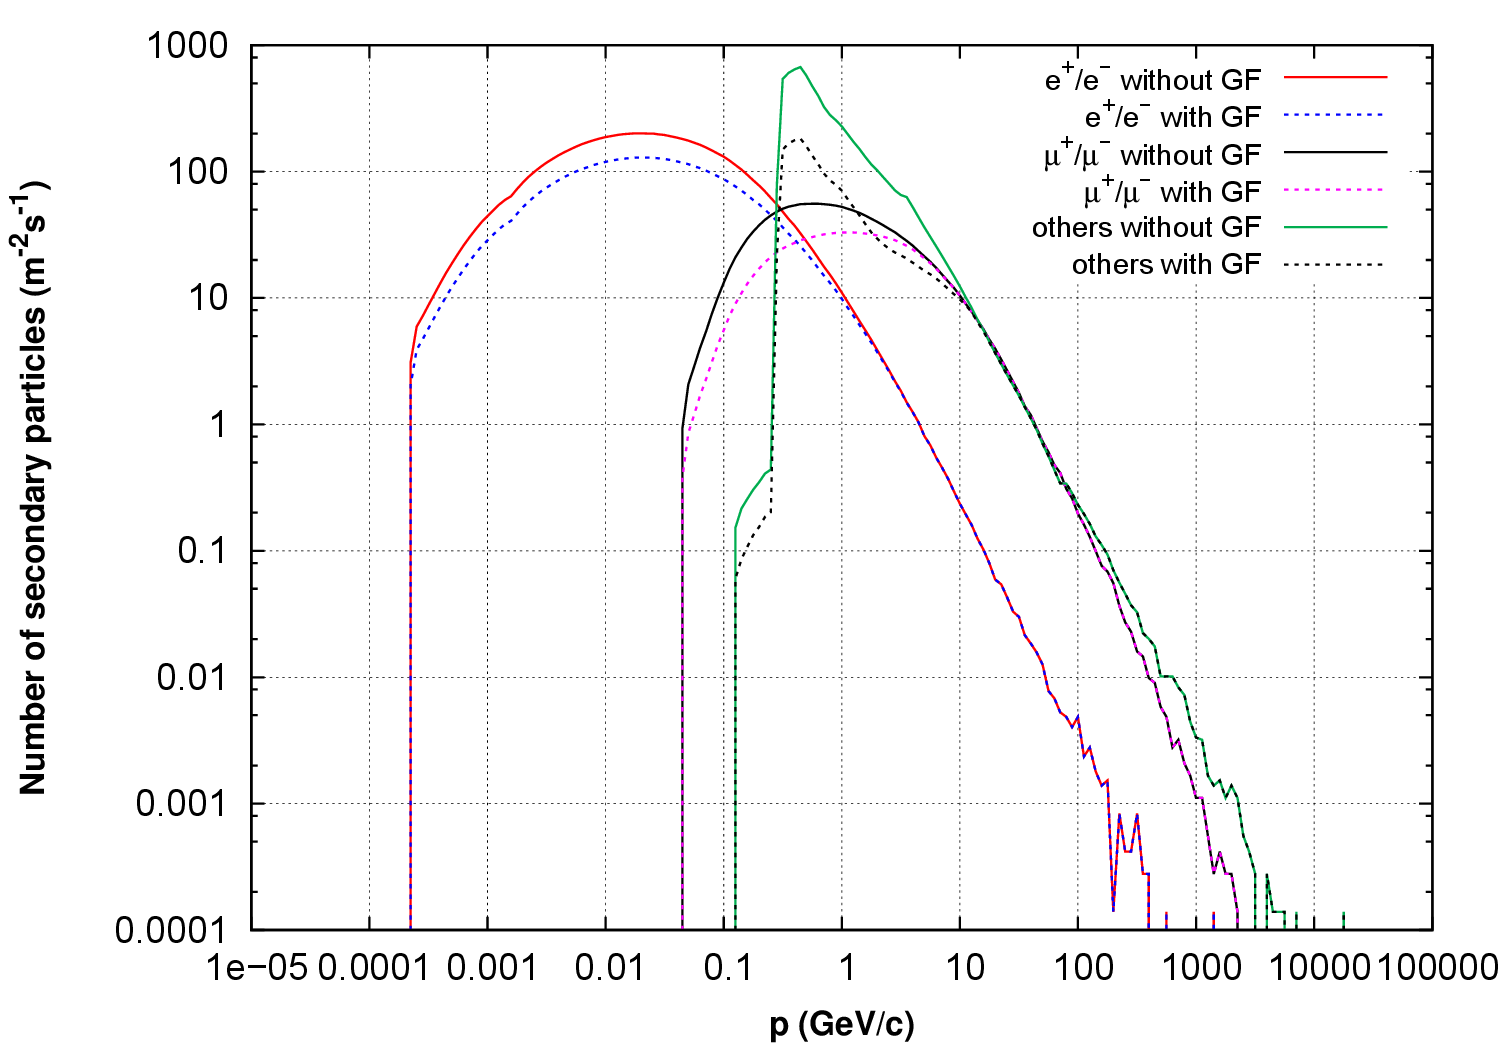
\includegraphics[scale=.14]{figures/g2_efectogeo2.png}
\caption{\textit{Distribution of particles considering the Geomagnetic Field  (dashed lines) and not considering it (continuous lines). Location: $14.74^\circ S\;67.27^\circ W$.}}
\label{fig:geo_effect2}
\end{figure}
\begin{figure}[H]
\centering
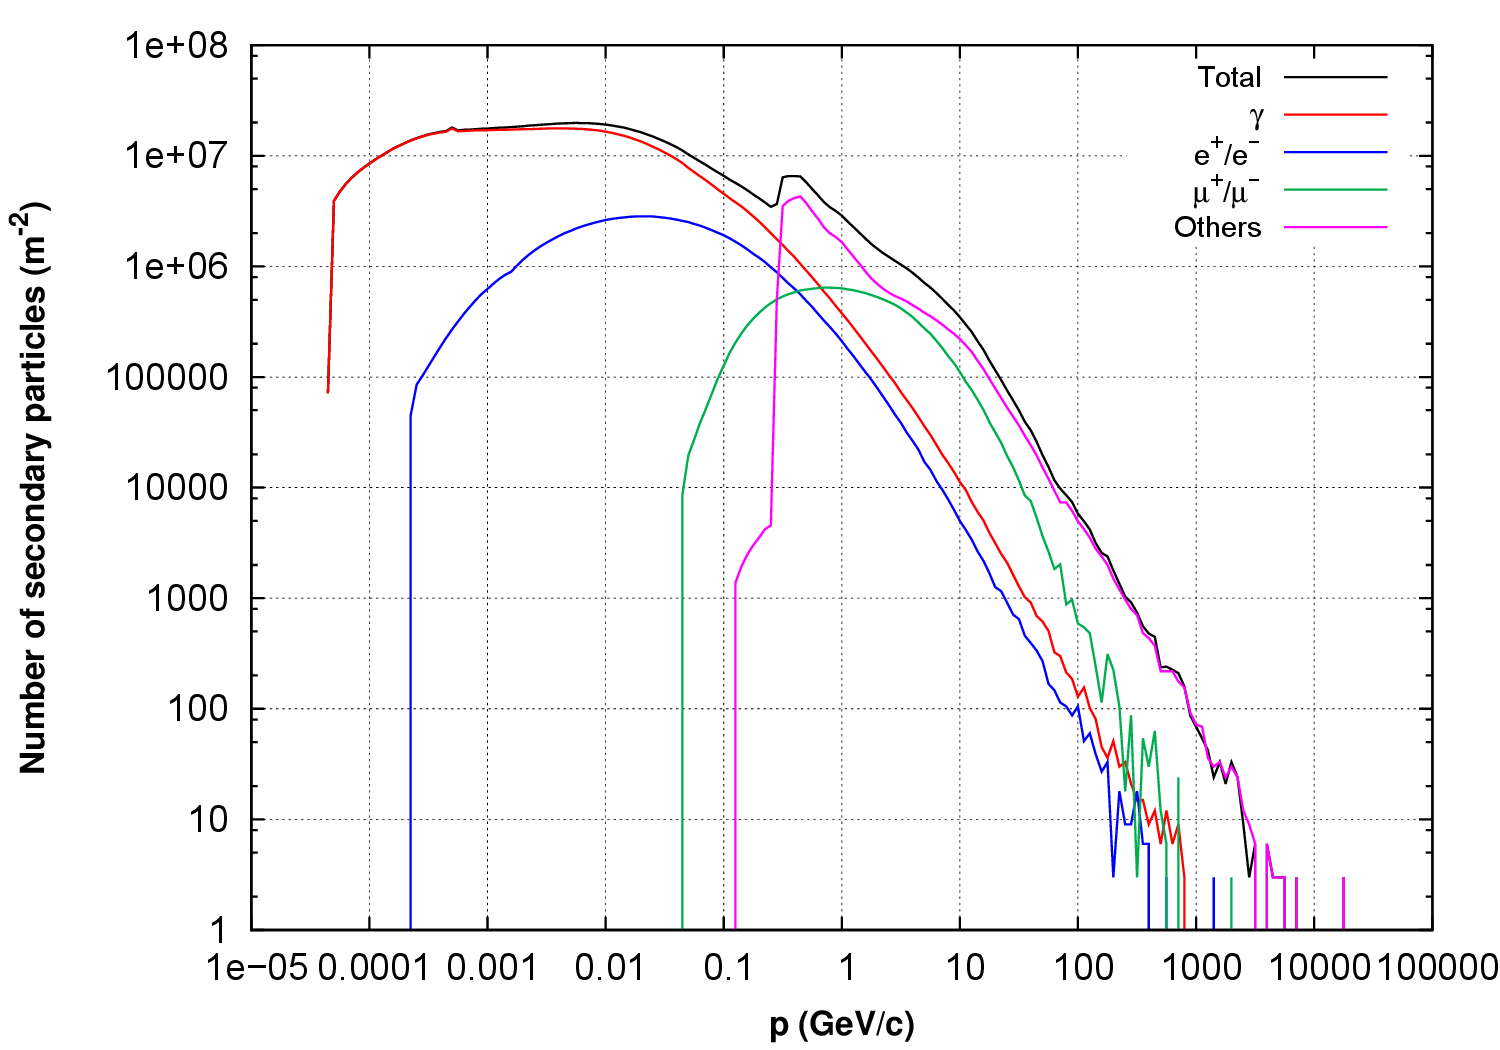
\includegraphics[scale=.14]{figures/g3_flujototal.png}
\caption{\textit{Distribution of particles during the flight Bogot\'a - Buenos Aires.}}
\label{fig:distribution_bta_bsas}
\end{figure}
\begin{figure}[H]
\centering
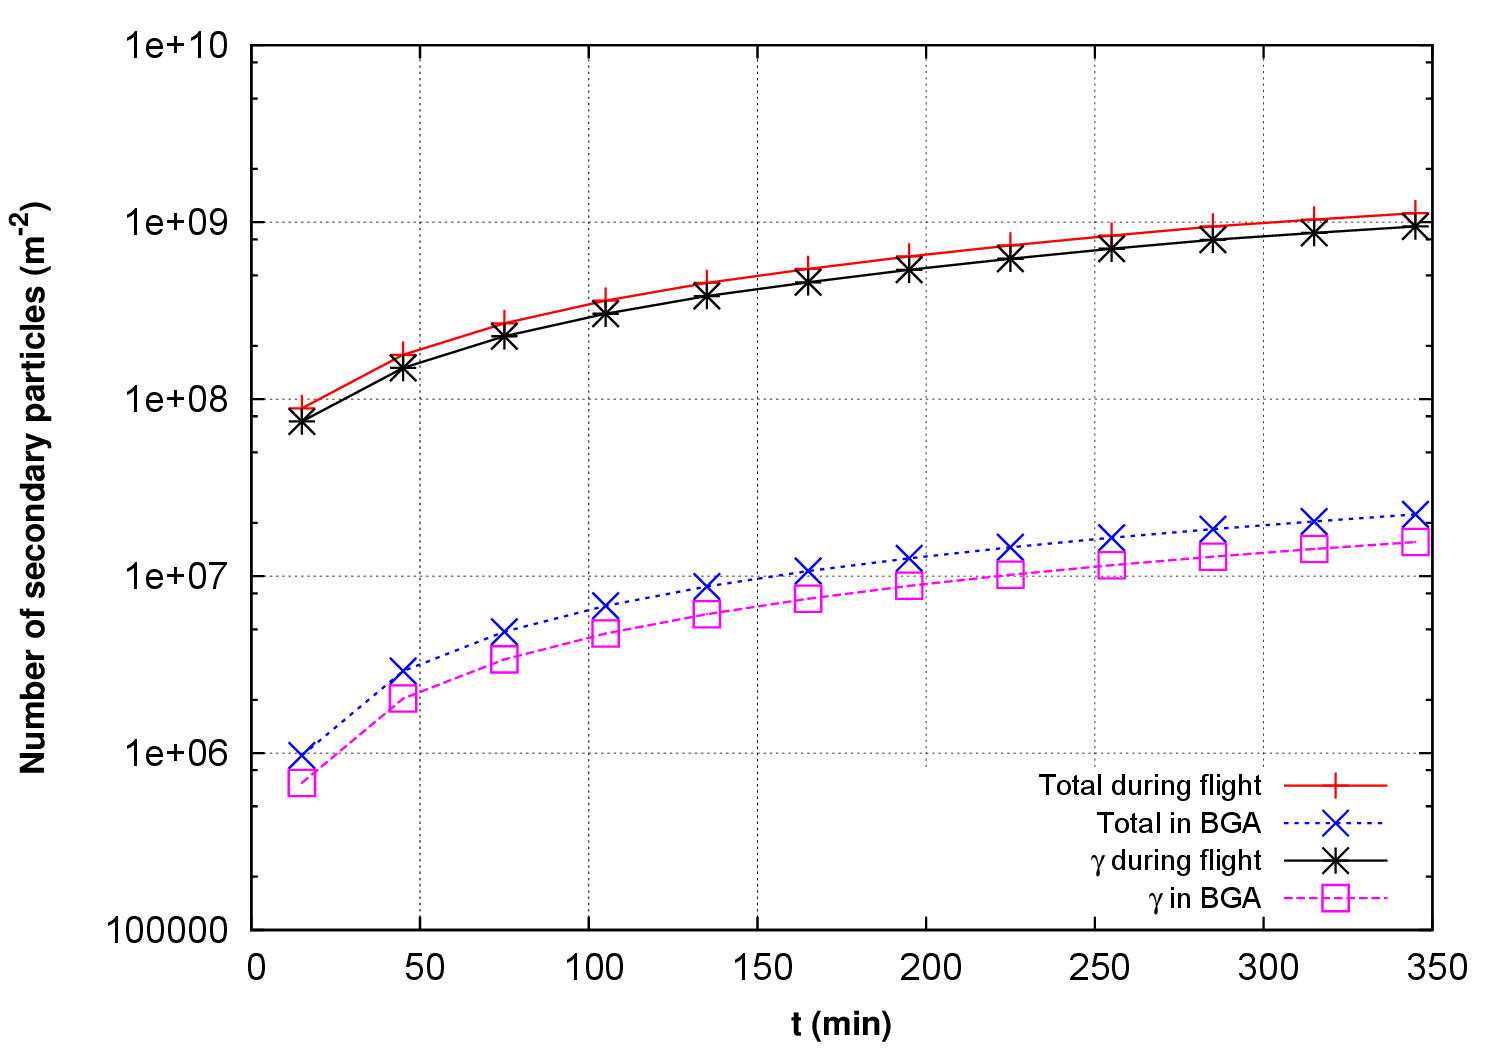
\includegraphics[scale=.14]{figures/g4_dosetime.png}
\caption{\textit{Integrated flux as function of time during the flight (continuous lines) and staying quiet in Bucaramanga (dashed lines).}}
\label{fig:integrated_bta_bsas}
\end{figure}

\section{Conclusions and acknowledgements}
\label{sec:conclusions}
The simulations performed show that at flight level, the number of secondary particles is two orders of magnitude greater than at 1000 m.a.s.l. When calculating the dose absorbed, geomagnetical effects must be taken into account since they reduce the number of primary particles that generate showers. To make more accurate calculations, aircraft's takeoff and landing will be included in the simulations. In order to study space weather effects, simulations will be performed including geomagnectic storm conditions. The authors of this work want to thank the support of COLCIENCIAS under the Grant 617/2014 "Semillero de  Investigaci\'on: Ciencia de datos y astropart\'iculas".
%% The Appendices part is started with the command \appendix;
%% appendix sections are then done as normal sections
%% \appendix

%% \section{}
%% \label{}

%% References
%%
%% Following citation commands can be used in the body text:
%% Usage of \cite is as follows:
%%   \cite{key}         ==>>  [#]
%%   \cite[chap. 2]{key} ==>> [#, chap. 2]
%%

%% References with BibTeX database:
%\nocite{*}
\bibliographystyle{elsarticle-num}
\bibliography{biblio_pinilla}

%% Authors are advised to use a BibTeX database file for their reference list.
%% The provided style file elsarticle-num.bst formats references in the required Procedia style

%% For references without a BibTeX database:

% \begin{thebibliography}{00}

%% \bibitem must have the following form:
%%   \bibitem{key}...
%%

% \bibitem{}

% \end{thebibliography}

\end{document}

%%
%% End of file `nuphbp-template.tex'. 